\section{Definition}
Als Sensoren werden Messfühler bezeichnet, welche z.B. optische, akustische, elektrische, magnetische oder auch stoffspezifische Signale empfangen und dies in einer verarbeiteten Form weiterleiten. Dabei ist die Reversibilität sehr wichtig.
\\Chemische Sensoren bestehen aus einem Stoffe erkennenden Teil und einem Messwertumwandler, der die Information im zu analysierenden Medium (Gas, Flüssigkeit) in ein elektrisches oder optisches Signal umändert.
\\Biochemische Sensoren enthalten eine biochemische oder biologische Komponente (Enzym, Antikörper, Zelle, Mikroorganismen) in Verbindung mit einem physikalisch-chemischen Messprinzip (Elektroden: Potenziometrie oder Amperometrie, Fluoreszenz u.a.).
\\Den Wechselwirkungsprozessen zwischen Analyt und Sensoren liegen physikalisch-chemische oder biochemische Mechanismen bzw. Prinzipien zugrunde:
\\Physiosorption, van der Waals-Kräfte und Chemisorption, Oberflächen-, Volumen-, Korngrenzen-, Grenzflächen- und Dreiphasen-Reaktionen, Reaktionen mit Käfigverbindungen und spezifische Reaktionen in Biosensoren.
\\Zu den physikalisch-chemischen Grundlagen der Analytik mit Sensoren gehören thermodynamische und kinetische Aspekte, angefangen von der Zustandsfunktion, dem Prinzip der Minimierung der freien Energie bzw. freien Enthalpie (Gibbs'sche Energie), der Berechnung der Zustandssumme, Berechnungen zur heterogenen Katalyse bis hin zur Aufstellung von Energiediagrammen und Funktionen zur Reaktionsgeschwindigkeit.
\\Man unterscheidet unter Verwendung der genannten thermodynamischen und kinetischen Grundlagen drei Arten von Sensorprinzipien: Gleichgewichtssensoren (thermodynamische Gleichgewichte), umsatzratenbestimmende Sensoren (unter kinetischen Fließgleichgewichtsbedingungen) und Einwegsensoren (ohne Reversibilität des Reaktionsprinzipes). \cite{[5]} %schwedt
%Reversibilität ist sehr wichtig, definition eines Sensors
\section{optische Sensoren}
Die Glasfasertechnik spielt bei der Entwicklung optischer Sensoren eine wichtige Rolle. Weil Glasfaserlichtleiter kleine Durchmesser aufweisen, begünstigt dies die Herstellung von Glasfaserlichtleitern, die bei der Konstruktion von in-vivo-Sensoren Anwendung finden. Mit diesen kann man z.B. in Körperflüssigkeiten messen. Der in vivo-pH-Optosensor auf faseroptischer Basis besteht aus einer kleinen Cellulose-Dialyseröhre, in der sich der Indikator Phenolrot (gebunden an Polyacrylamid-Partikel) und etwa 1 \textmu m große Polystyrolkügelchen als Füllung befinden. Die Dialyseröhre ist direkt an ein Lichtleiterpaar aus Kunststoff gekoppelt. Das eingestrahlte Licht wird an den Polystyrol-Kugeln (Indikatorkugeln), die mit Körperflüssigkeit in Kontakt stehen, gestreut und ändern ihr Lichtabsorptionsverhalten in Abhängigkeit vom pH-Wert. Das über die zweite Lichtfaser zurückgestrahlte Licht wird schließlich auf eine Photodiode übertragen. \cite{[5]}
%gibt es auch in Polymer siehe Klimant/Mayr oder A.Mills

\subsection{Faseroptische Sensoren}
Diese Art von Sensoren findet auch Einsatz in Fließsystemen. Durch Remissionsmessung ( Wiederaussendung von einfallenden Wellen oder Teilchen) werden die pH-abhängigen Absorptionsänderungen bestimmt.
Bei Faseroptischen Sensoren in Polymeren wird der Lumophor in Silica-Gel-Kugeln integriert und getrocknet. Dann wird er mit einem Silicon-Prepolymer homogen vermischt, für 12 h bei 40°C ausgehärtet. Das Silkon wird dann in heißes Wasser getaucht um  es zu füllen. Das in den Sensor eindiffundierte Wasser verändert die Polarität in Umgebung des Farbstoffes. Dies führt zu einer kontinuierlichen hypsochromen Verscheibung der Absorption in Abhängigkeit vom Wassergehalt. \cite{[6]} %mills
Beim Ammoniak-Optosensor  wird der Analytstrom vom Indikatorsystem getrennt (durch eine weiße permeable Teflon-Membran) und kann so kontinuierlich gemessen werden. Die Änderung der Farbe, die an der Grenzfläche auftritt, kann ermittelt werden. Die Fluorometrie wird genauso wie die Photometrie in Optosensoren verwendet. Lichtleiter können auch direkt chemisch beschichtet werden. An einem Ende wird der Lichtleiter mit Licht einer Leutdiode durchstrahlt, und wird mittels Photodiode registriert. Beim Durchstrahlen der gassensitiven Beschichtung wird der Grenzwinkel eingehalten, um  eine intern an der Grenzschicht Polymer/Luft zu reflektrieren. Wenn Moleküle des Analyten die Schicht durchwandern setzen sie sich mit der vorhandenen Reagenz. Der intern reflektierte Lichtstrahl wird somit abgeschwächt.\cite{[5]}
%andere Formen planare Optode, imaging mit CCD-Kamera, Nanopartikel
\\Bei planaren Optoden basiert die Messung auf der Verwendung von spezifischen Fluoreszenzfarbstoffen, die kurzfristig mit Licht einer oder mehrerer spezieller Wellenlängen angeregt werden. Der Farbstoff wird in einer Polymermatrix fixiert und auf das untersuchende Medium aufgebracht. Die Messung erfolgt z.B. mit CCD-Kamera außerhalb des Mediums. Damit ist auch nicht-invasive Erfassung möglich. %googlecite
\subsection{optothermische Sensoren}
Neben den oben vorgestellten Sensoren werden auch optothermische (photoakustische) Sensoren eingesetzt. Materie wird mit Licht z.B. im IR-Bereich für $CO_2$ oder $NO_2$ Analysen bestrahlt wird und wenn die IR-Strahlung absorbiert wird, so vergrößert sich das Gasvolumen und dieser Druckanstieg stellt das Messsignal dar. \cite{[5]}
\section{optische Sauerstoffsensoren}
In Wissenschaft und Technik spielt Sauerstoff als Analyt eine wichtige Rolle. Dies kann über optische Sensoren, die nichtinvasiv oder minimal invasiv (invasiv= in Gewebe eindringend) und austauschbar sind, überprüft werden. Sie können leicht verkleinert werden und die Sauerstoffdichte in einem Volumen oder über einer Oberfläche messen. Als UV-Vis Sauerstoffindikatoren werden vor allem luminiszierende Metallkomplexe verwendet, z.B. Ruthenium(II)polypyridyl-Komplexe, Platin(II) und Palladium(II)-Porphyrine oder Iridium(III)-Coumarine. \cite{[6]}
\\Das Messprinzip eines optischen Sauerstoffsensors basiert auf der optischen Messung der Sauerstoffkonzentration. Auf die Spitze eines optischen Kabels wird ein chemischer Film geklebt, der die Phosphoreszenzeigenschaften misst, die von der Sauerstoffkonzentration abhängen. Die Phosphoreszenz ist am Maximum, wenn kein Sauerstoff vorhanden ist. Wenn $O_2$-Moleküle mit dem Film zusammenstossen, löschen sie die Photolumineszenz aus. In einer festgelegten Sauerstoffkonzentration werden bestimmt viele $O_2$-Moleküle mit dem Film zu jeder Zeit zusammenstossen und die Phosphoreszenz-Eigenschaften werden stabil sein.
\\Das Signal-Sauerstoff-Verhältnis ist nicht linear und eine Optode ist am empfindlichsten, wenn die Sauerstoffkonzentration niedrig ist. Das heißt, dass die Empfindlichkeit sinkt, wenn die Sauerstoffkonzentration steigt. Der Optodensensor kann im gesamten Bereich von 0-100$\%$ Sauerstoffsättigung im Wasser arbeiten.
%kann man auch graphisch zeigen; Stern-Volmer-gleichung ist wichtig
\begin{figure}[!htpb]
\centering
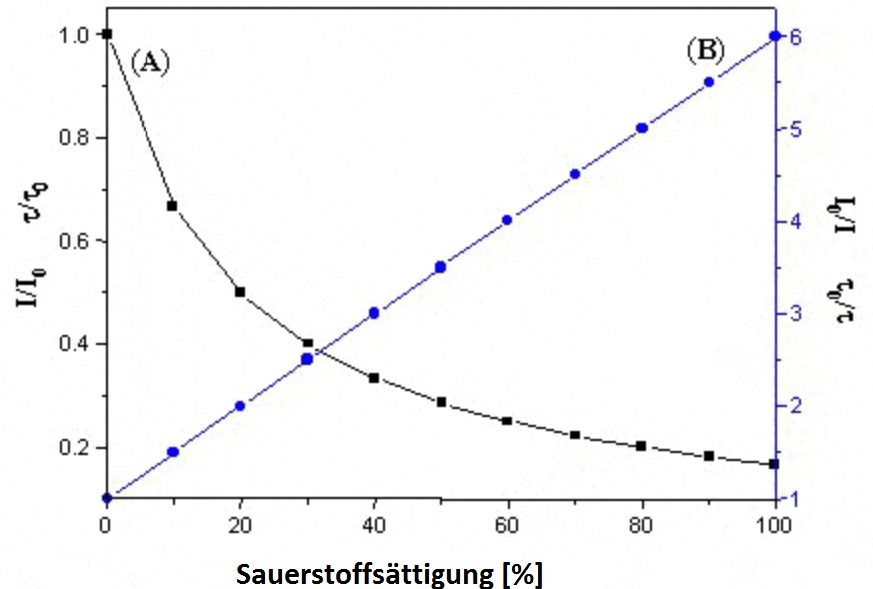
\includegraphics[scale=0.5]{graphics/stern-volmer}
\caption{(A) Lumineszenzabnahme in Gegenwart von Sauerstoff; (B) Stern-Volmer-Plot}

\end{figure}
 Kein Sauerstoff wird verbraucht und deswegen ist der Sensor unempfindlich gegenüber Rührung (diese kann das Signal schneller stabilisieren). Diese Art von Sensor kann für in-situ und Echtzeit- Beobachtung der Sauerstoffproduktion in Wasserabspaltenden Reaktionen benutzt werden. \cite{[7]}
\\Die oben beschriebenen Sauerstoffsensoren haben auch Grenzen. Diese Sensoren können nicht in mehrfachstreuenden und fluoreszierenden Materialien (z.B.Chlorophyll) enthaltenden Medien benutzt werden. UV-Vis Indikatoren sind nicht für Messungen in Unterhautgewebe geeignet, weil es zu hohen Streuverlusten kommt und weil Blut Licht im sichtbaren Bereich absorbiert.
\\Dafür können NIR-Sauerstoff-Indikatoren verwendet werden, die den Vorteil haben, weniger zu streuen, weniger Autofluoreszenz zu haben und das Messungen im Gewebe möglich sind \cite{[6]} %borisov
\subsection{Implantierbare Glukose-Sensoren}
%Prinzip erklären; Gleichung
Das Prinzip dieser Sensoren ist, dass Glukose in Gegenwart von Sauerstoff und Wasser  von dem Enzym Glukose-Oxidase zu Gluconolacton umgewandelt wird und die Abnahme des Sauerstoffs gemessen wird:
\\\ce{Glukose + O2 + H2O ->T[Glukose][oxidase] Gluconolacton + H2O2}
\\Implantierbare Glukose-Sensoren könnten bei der Diabetes-Überwachung helfen und verlassen sich auf Sauerstoffindikatoren als Transduktoren. Sie sollen unter der Haut implantiert werden und vitale Analyten wie Glukose oder Sauerstoff überwachen. Solche "Tattoos" werden über die Haut angeregt und interagieren mit einer Photodiode oder einer CCD-Kamera.  \cite{[6]}
\begin{figure}[htpb]
\centering
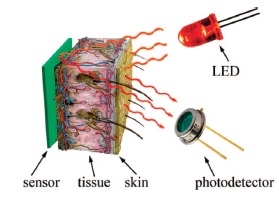
\includegraphics[scale=1]{graphics/Glucose-Sensor}
\caption{Aufbau eines Implantierbaren Glucosesensors}
\end{figure}
